\documentclass[12pt]{article}
\usepackage{hyperref}
\usepackage{listings}
\usepackage[margin=1in]{geometry}
\usepackage{enumitem}
\usepackage{multicol}
\usepackage{array}
\usepackage{titlesec}
\usepackage{helvet}
\renewcommand{\familydefault}{\sfdefault}
\usepackage{amsmath}     % For math equations
\usepackage{amssymb}     % For advanced math symbols
\usepackage{amsfonts} % For math fonts
\usepackage{gvv}
\usepackage{esint}
\usepackage[utf8]{inputenc}
\usepackage{graphicx}
\usepackage{pgfplots}
\pgfplotsset{compat=1.18}
\titleformat{\section}{\bfseries\large}{\thesection.}{1em}{}
\setlength{\parindent}{0pt}
\setlength{\parskip}{6pt}
\usepackage{multirow}
\usepackage{float}
\usepackage{caption}





\begin{document}

\textbf{Problem 1.4.2 .}  
Find the coordinates of the point \(R\) on the line segment joining
P(1,3) and Q(2,5) such that $\vec{PR}=\dfrac{3}{5}\,\vec{PQ}$


\textbf{Solution.}  

\begin{table}[H]
\centering
\begin{tabular}[12pt]{ |c| c|}
    \hline
    \textbf{Input variable} & \textbf{Value}\\ 
    \hline
    $\vec{P}$ & \myvec{1 \\3 } \\
    \hline 
    $\vec{Q}$ & \myvec{2 \\ 5}\\
    \hline
    $\frac{PR}{PQ}$ & $\frac{3}{5}$\\
    \hline
    \end{tabular}
    \caption{
    \label{}
    }
 \end{table}
Let the position vectors be
$$
\vec{P} = \myvec{1 \\ 3}, \qquad
\vec{Q} = \myvec{2 \\ 5}.
$$
If \(\vec{R}\) is the position vector of \(R\), then
$$
\vec{R} - \vec{P} = \frac{3}{5}(\vec{Q} - \vec{P})
\;\;\Longrightarrow\;\;
\vec{R} = \vec{P} + \frac{3}{5}(\vec{Q} - \vec{P}).
$$
So,
$$
\vec{R}
= \myvec{1 \\ 3}
+ \frac{3}{5}\left(\myvec{2 \\ 5} - \myvec{1 \\ 3}\right)
= \myvec{1 \\ 3} + \frac{3}{5}\myvec{1 \\ 2}.
$$
Hence,
$$
\vec{R} = \myvec{1+\tfrac{3}{5} \\[4pt] 3+\frac{6}{5}}
= \myvec{\frac{8}{5} \\[6pt] \frac{21}{5}}.
$$

Therefore, the required point is
$$
\boxed{\;\vec{R} = \myvec{\frac{8}{5} \\[6pt] \frac{21}{5}}\;}
$$
which indeed satisfies \(\vec{R} - \vec{P} = \frac{3}{5}(\vec{Q} - \vec{P})\).

\begin{figure}[H]
    \centering
    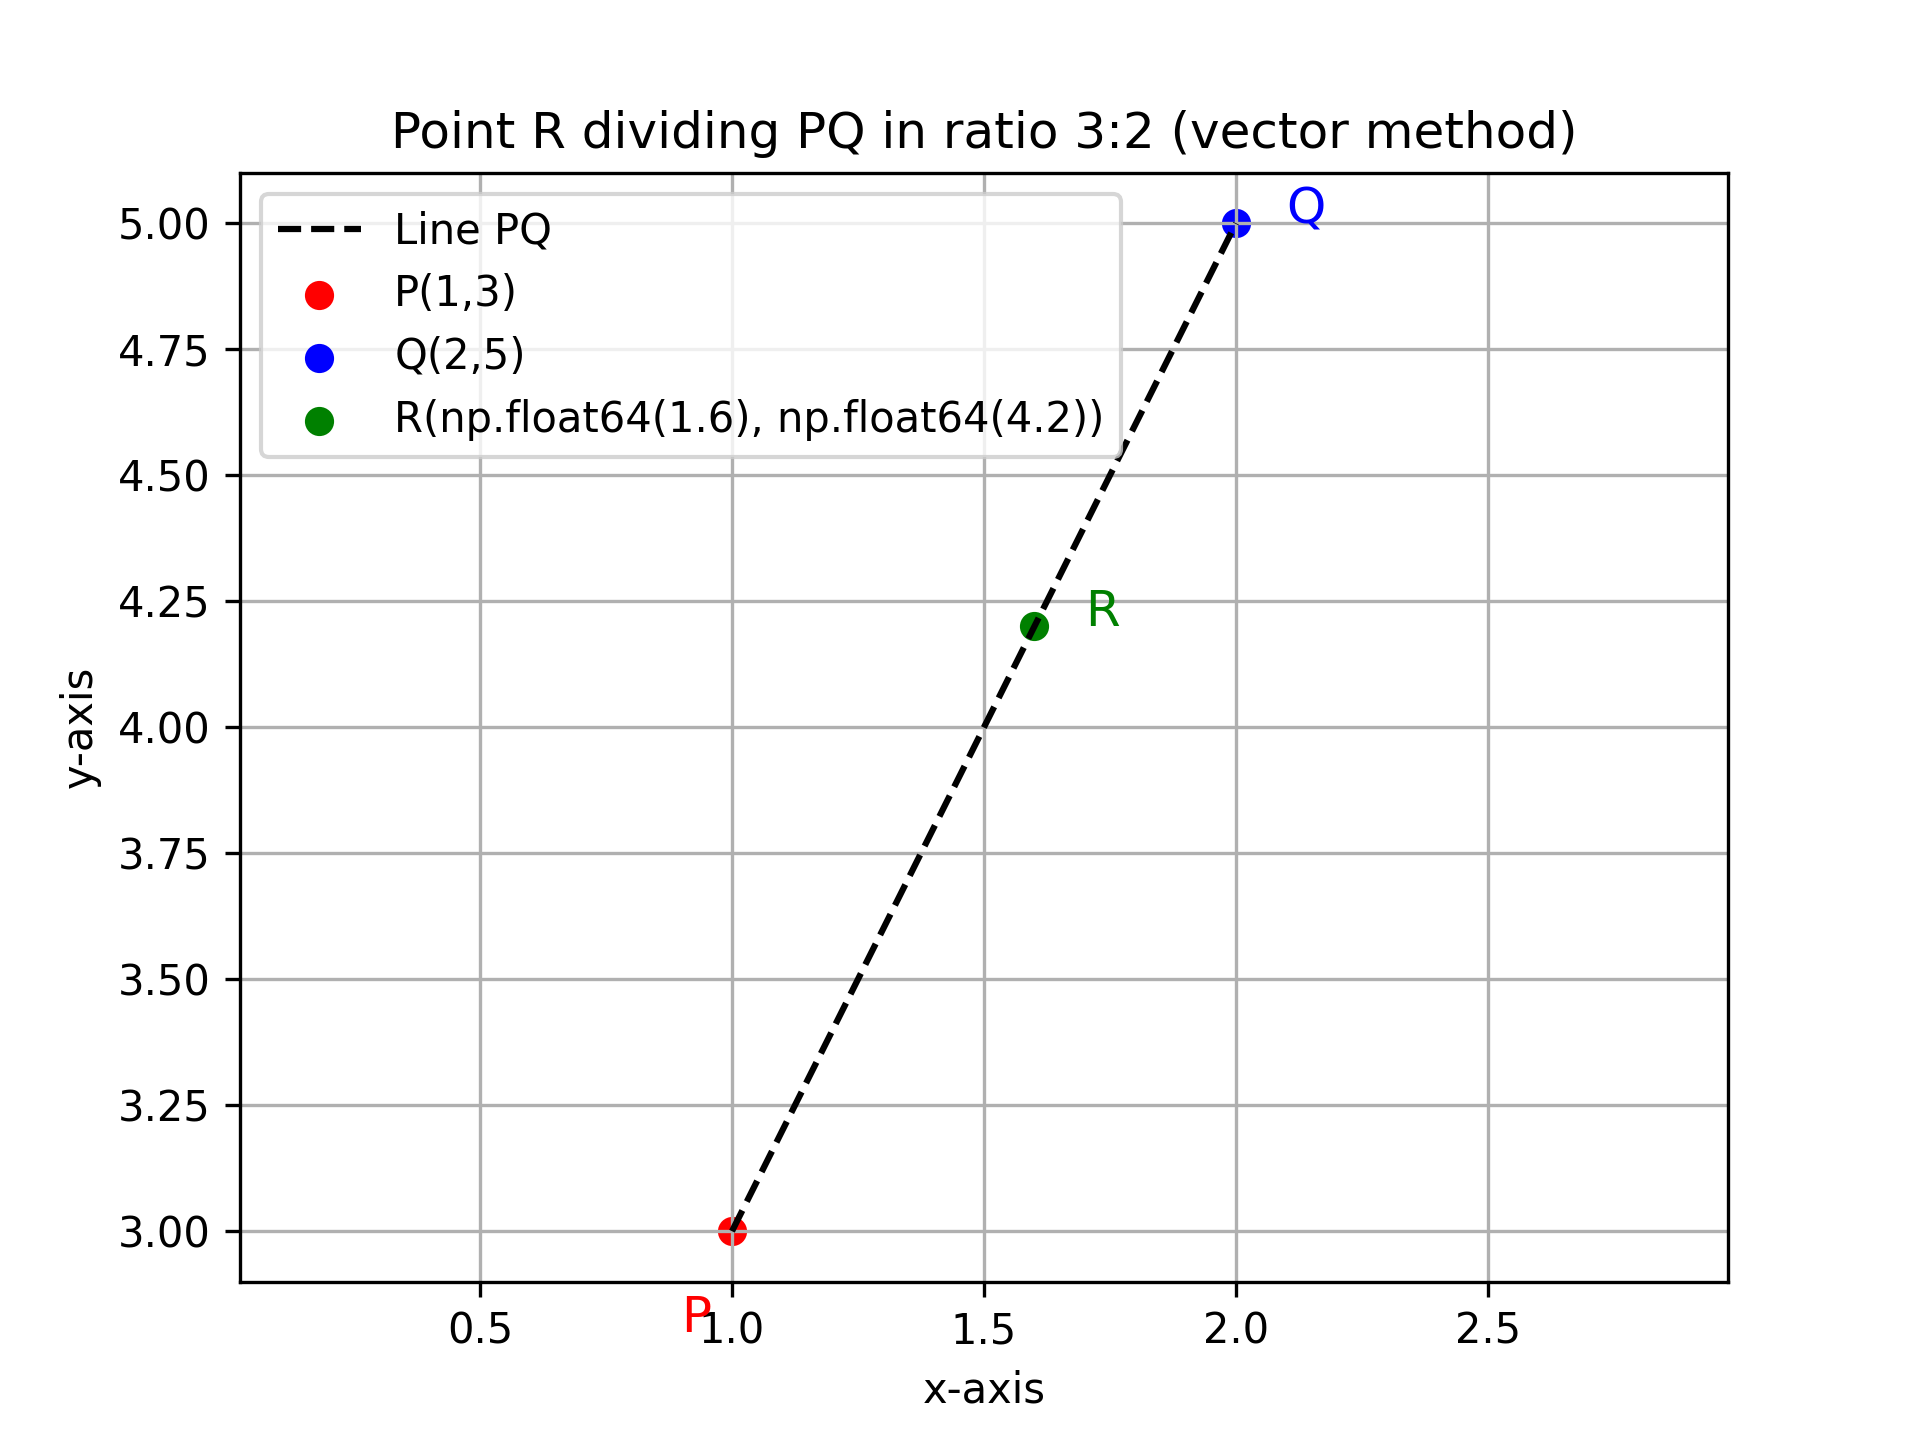
\includegraphics[width=1\columnwidth]{figs/PQ_R_plot.png}
    \caption{}
    \label{fig:placeholder}
\end{figure}
\end{document}




